\section{Методика верификации}

Предлагаемая методика верификации основана на сопоставлении трасс исполнения
распределённой реализации с формальной спецификацией, написанной на языке TLA+.
Общая схема подхода представлена на рисунке~\ref{fig:arch}.

\begin{figure}
  \centering
  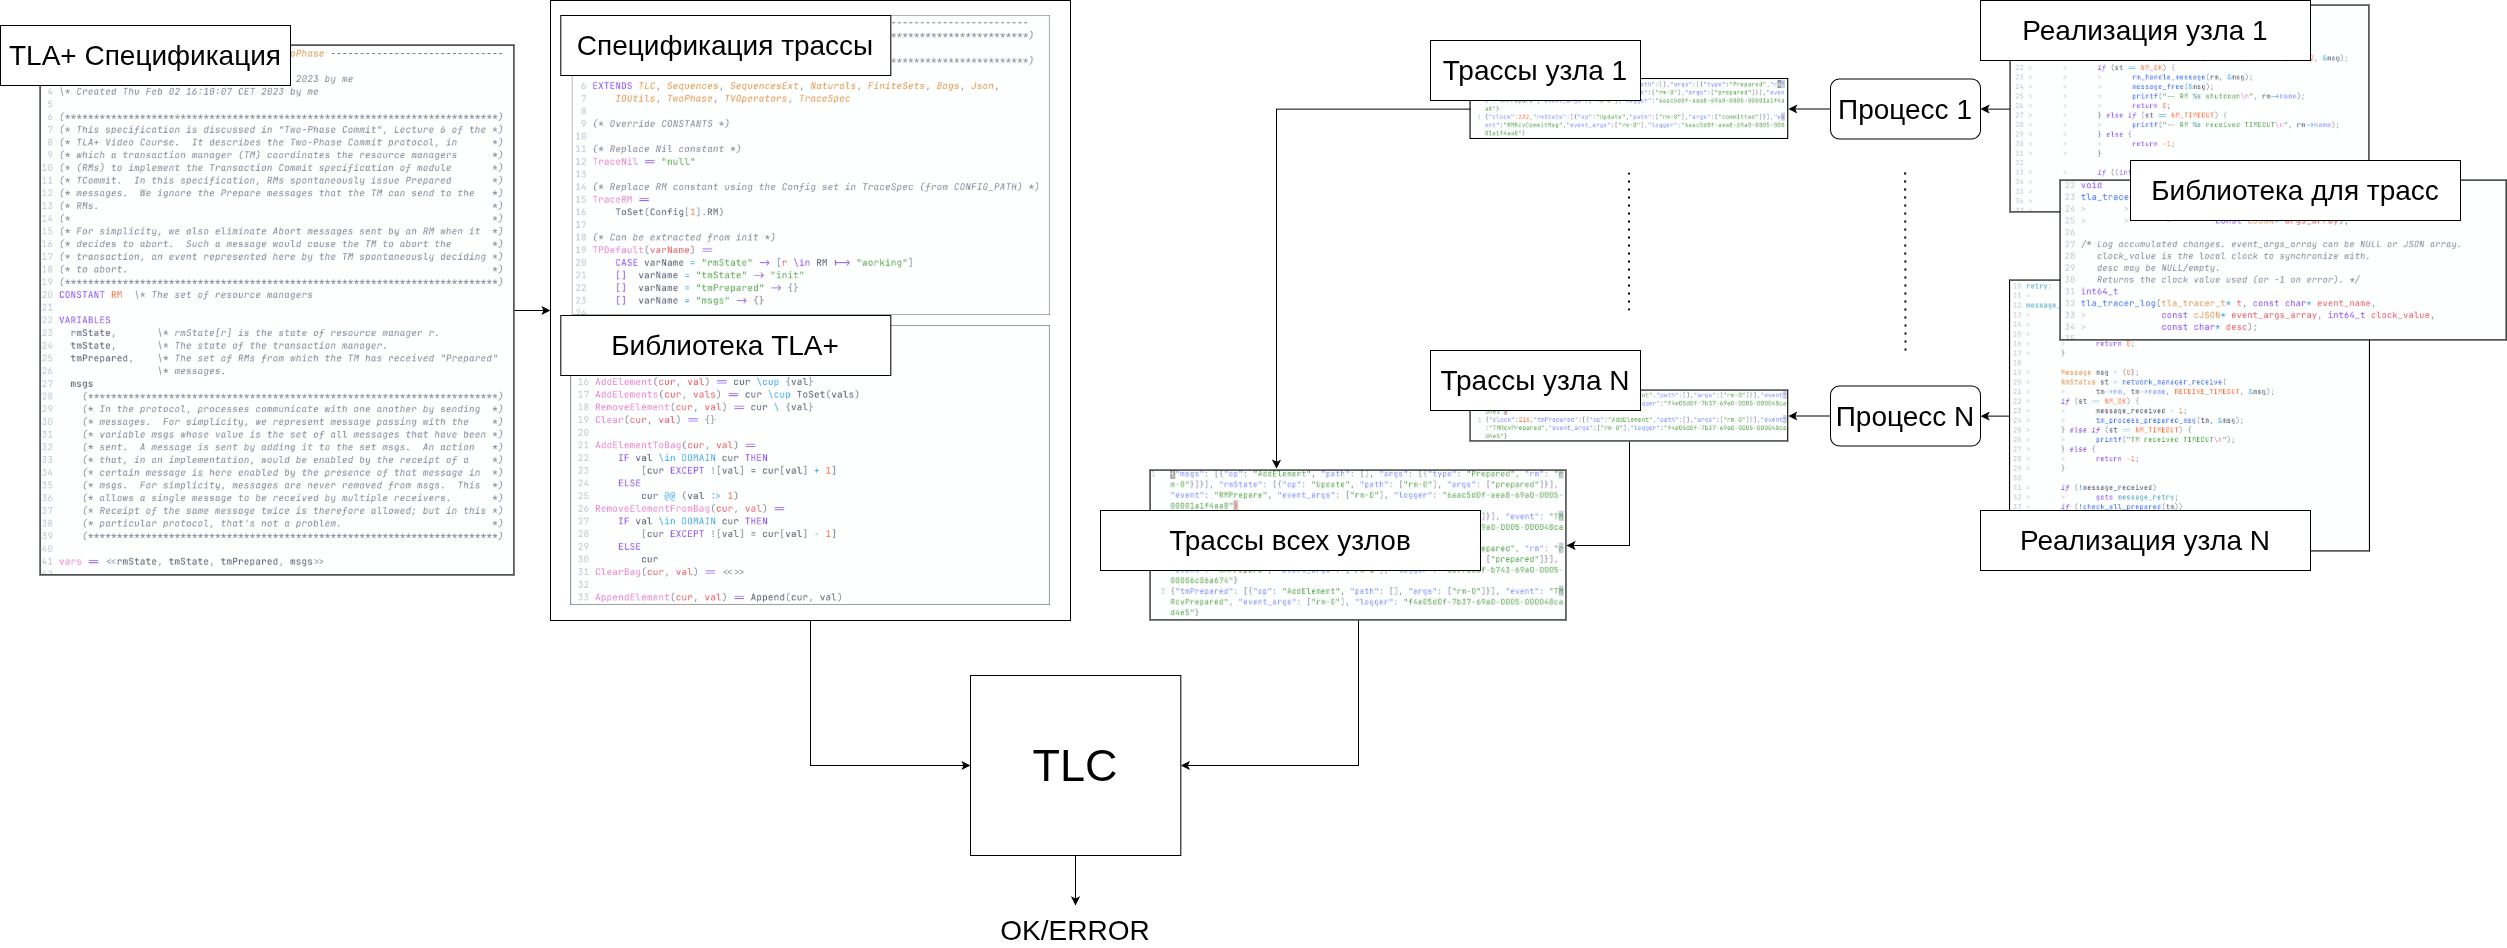
\includegraphics[scale=0.17]{inc/arch.png}
  \caption{Методика верификации}
  \label{fig:arch}
\end{figure}

Исходными артефактами являются:

\begin{itemize}
    \item программная реализация алгоритма.
    \item формальная спецификация этого алгоритма на языке TLA+.
\end{itemize}

Спецификация задаёт множество допустимых состояний системы и переходов между
ними, однако не содержит сведений о конкретной реализации. Реализация, в свою
очередь, выполняется в распределённой среде, где возможны различные порядки
доставки сообщений и недетерминированные сценарии выполнения.

Для сопоставления поведения реализации со спецификацией используется
инструментирование кода. В реализацию внедряется библиотека трассировки,
которая фиксирует события, соответствующие переходам спецификации, а также
изменения переменных спецификации. При выполнении системы каждый процесс
(координатор и участники) формирует собственную трассу в формате JSON,
содержащую последовательность операций обновления логических переменных модели.

Полученные локальные трассы агрегируются в единый глобальный файл, отражающий
наблюдаемую последовательность изменений состояния всей распределённой системы.
Таким образом, формируется абстрактное представление исполнения, выраженное в
терминах переменных TLA+, а не в терминах низкоуровневых операций кода.

Для проверки корректности трассы используется дополнительная спецификация
(Trace Specification), построенная на основе исходной TLA+ спецификации. Она
расширяет её таким образом, чтобы поведение модели было ограничено наблюдаемой
последовательностью изменений. Иными словами, трасса интерпретируется как
частичное ограничение на допустимые переходы модели.

Далее средство модельной проверки TLC используется для проверки существования
поведения спецификации, согласованного с данной трассой. Если TLC подтверждает
корректность, это означает, что наблюдаемое исполнение допустимо спецификацией.
В противном случае обнаруживается расхождение между реализацией и моделью, и
TLC предоставляет контрпример, позволяющий локализовать проблему.

\subsection{Задача валидации трасс}

Задача валидации трасс формулируется следующим образом. Пусть $S$ ---
множество конечных поведений, удовлетворяющих спецификации $Spec$, и пусть
$T$ --- множество конечных поведений, представляемых трассой исполнения,
где переменным, значения которых не были зафиксированы в трассе,
разрешается принимать произвольные значения. Трасса считается совместимой
со спецификацией тогда и только тогда, когда
\[
S \cap T \neq \varnothing.
\]
Иными словами, существует хотя бы одно поведение спецификации,
согласующееся с наблюдаемой трассой. Заметим, что мы не проверяем условие
уточнения (refinement) высокоуровневой спецификации трассой, выражаемое
как $T \subseteq S$. Такое условие было бы слишком строгим в случае,
когда значения некоторых переменных не фиксируются в трассе и могут
выбираться недетерминированно.

Рис~\ref{fig:traces-search} иллюстрирует идею. Слева изображается линейная
цепочка состояний, соответствующая трассе, полученной из инструментированной
реализации. Справа --- граф состояний, определяемый спецификацией TLA+.
Требуется проверить, существует ли в графе состояний спецификации путь, который
можно сопоставить данной трассе.

\begin{figure}
  \centering
  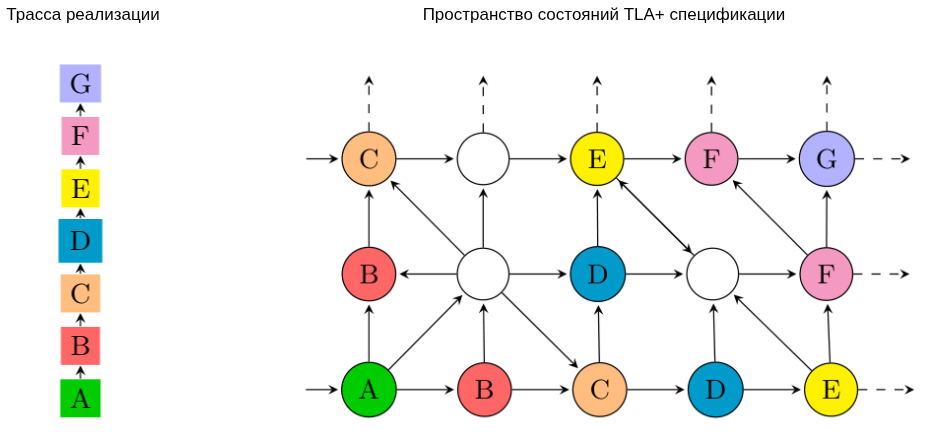
\includegraphics[scale=0.5]{inc/traces-search.png}
  \caption{Валидация трассы как поиск пути в пространстве состояний}
  \label{fig:traces-search}
\end{figure}

Первое состояние трассы должно соответствовать некоторому начальному состоянию
спецификации. Далее для каждого последующего шага трассы необходимо найти хотя
бы одного преемника уже сопоставленного состояния, который соответствует
следующему элементу трассы. Из-за неполной информации о значениях переменных
одному шагу трассы может соответствовать несколько состояний спецификации. Если
для некоторого состояния спецификации не существует допустимого продолжения,
согласующегося со следующим элементом трассы, такая ветвь поиска отбрасывается.
Трасса признаётся совместимой, если существует по крайней мере один путь в
графе состояний спецификации, который полностью соответствует всей
последовательности шагов трассы.

Следует учитывать дополнительную тонкость: атомарные шаги реализации не обязаны
в точности совпадать с атомарными переходами спецификации. Один шаг программы
может соответствовать нескольким шагам TLA+ или, наоборот, некоторым переходам
спецификации может не соответствовать явного события в трассе. Поэтому задача
валидации сводится к проверке существования пути в пространстве состояний
спецификации при дополнительных ограничениях, задаваемых трассой. Практически
эта редукция реализуется с помощью модельного проверяющего TLC.

В общем случае разработчик должен явно задать соответствие между
именами событий в трассе и действиями спецификации, а также между
именами логируемых переменных и переменными TLA+.

\subsection{Реализация инструментирования спецификации}

Множество $S$ конечных поведений, удовлетворяющих исходной спецификации,
задаётся формулой TLA+ $Spec$. Для того чтобы охарактеризовать пересечение $S
\cap T$, то есть поведения спецификации, совместимые с трассой исполнения, к
спецификации добавляются дополнительные ограничения. Таким образом, задача
сводится к построению ограниченной спецификации, учитывающей информацию из
трассы.

В разработанном фреймворке для этого используется отдельный модуль
\texttt{TraceSpec}, предоставляющий операторы для построения ограниченной
версии исходной спецификации. Его часть приведена на
рис.~\ref{fig:trace-spec-1}.

\begin{figure}
  \centering
  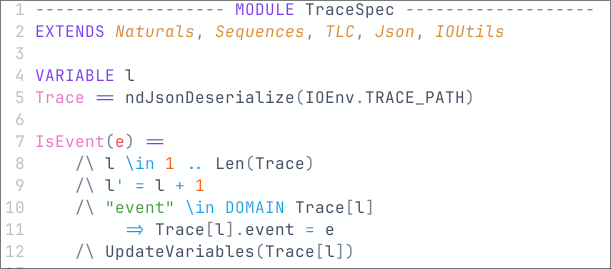
\includegraphics[scale=0.5]{inc/trace-spec-1.png}
  \caption{Реализация $IsEvent()$ из модуля $TraceSpec$}
  \label{fig:trace-spec-1}
\end{figure}

Модуль объявляет переменную $l$, обозначающую номер текущей строки трассы.
Оператор $Trace$ десериализует NDJSON-файл и представляет трассу программы в
виде последовательности записей, каждая из которых соответствует одной записи
журнала исполнения.

Оператор $IsEvent(e)$ инкапсулирует обработку текущей строки трассы.
Он проверяет, что индекс $l$ корректен, увеличивает его на единицу и,
если в записи явно указано поле \texttt{"event"}, проверяет соответствие
ожидаемому имени действия. Параметры события, если они заданы, учитываются
далее. Кроме того, вызывается оператор $UpdateVariables$ (см.
рис~\ref{fig:trace-spec-2}, который накладывает ограничения на значения
переменных спецификации.

\begin{figure}
  \centering
  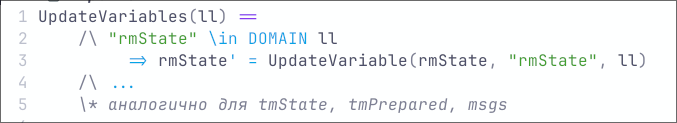
\includegraphics[scale=0.5]{inc/trace-spec-2.png}
  \caption{Реализация $UpdateVariables()$}
  \label{fig:trace-spec-2}
\end{figure}

Данный оператор проверяет, присутствует ли в текущей строке трассы обновление
соответствующей переменной. Если да, новое значение вычисляется с помощью
вспомогательного оператора $UpdateVariable$ (также определенного в
\texttt{TraceSpec}), который принимает старое значение переменной и описание
операции из JSON-записи.

Для каждого действия исходной спецификации строится соответствующее
действие ограниченной спецификации, получаемое конъюнкцией с
предикатом $IsEvent$. Пример приведен на рис.~\ref{fig:trace-spec-3}

\begin{figure}
  \centering
  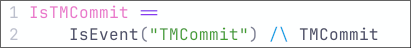
\includegraphics[scale=0.5]{inc/trace-spec-3.png}
  \caption{Пример действия ограниченной спецификации}
  \label{fig:trace-spec-3}
\end{figure}

Поскольку TLC вычисляет формулы слева направо, сначала применяются ограничения
из трассы (обновляются переменные), после чего проверяется, удовлетворяет ли
полученное состояние предикату действия исходной спецификации. Для переменных,
значения которых не зафиксированы в трассе, TLC может недетерминированно
выбирать подходящие значения.

Для параметризованных действий учитываются аргументы, указанные в трассе.
Например:

Таким образом, если в трассе указан конкретный параметр, рассматривается
соответствующий экземпляр действия; иначе TLC разрешается выбрать любой
допустимый параметр.

Общее отношение перехода ограниченной спецификации $TraceNext$ определяется как
дизъюнкция всех таких ограниченных действий. Построение этой спецификации в
большинстве случаев является систематическим и может быть автоматизировано.

При проверке TLC вычисляет все возможные преемники текущего состояния. Даже
если из некоторого состояния нельзя продолжить сопоставление с трассой, в
пространстве состояний могут существовать другие ветви, соответствующие трассе.
Поэтому не следует включать проверку deadlock для ограниченной спецификации.

Для валидации трасс использовать постусловие, приведенное на
рис.~\ref{fig:trace-spec-4}.

\begin{figure}
  \centering
  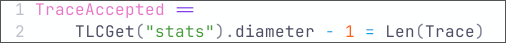
\includegraphics[scale=0.5]{inc/trace-spec-4.png}
  \caption{Условие валидации соответствия трасс}
  \label{fig:trace-spec-4}
\end{figure}

Если данное условие выполняется, существует поведение спецификации, полностью
соответствующее трассе. Если нет, пересечение $S \cap T$ пусто, и трасса
несовместима со спецификацией. В этом случае TLC не может предоставить единый
контрпример (поскольку подходящего поведения не существует), однако может
вывести максимальный префикс поведения спецификации, совпадающий с трассой.

Следует отметить, что при неполной трассировке возможны ложноположительные
результаты: если трасса содержит слишком мало информации (например, фиксирует
только длину исполнения без обновлений переменных и имён действий), модельный
проверяющий может недетерминированно подобрать значения переменных так, что
будет найдено совместимое поведение. Поэтому степень детализации трассировки
напрямую влияет на точность валидации и размер пространства поиска.

\subsection{Библиотека инструментирования реализации}

Для сопоставления поведения реализации с формальной спецификацией TLA+ была
разработана библиотека инструментирования на языке~C \cite{tlacimpl}. Её задача
--- фиксировать изменения логических переменных модели и формировать трассу
исполнения в формате NDJSON, пригодную для последующей валидации средствами
TLC.

Библиотека реализует следующий принцип:

\begin{enumerate}
    \item Во время выполнения программы фиксируются изменения логических
    переменных спецификации через \texttt{notify\_change}.
    \item В точке линейризации вызывается \texttt{log}, формируя
    атомарную запись трассы.
    \item Полученный NDJSON-файл представляет последовательность
    логических шагов, которые могут быть сопоставлены с действиями
    TLA+ спецификации.
    \item Полученные от разных процессов трассы можно объединить, используя
Python скрипт \texttt{trace\_merger.py}.
\end{enumerate}

Библиотека предоставляет абстракцию \texttt{tla\_tracer\_t}, инкапсулирующую
логику накопления изменений переменных и формирования записей трассы. Основной
интерфейс представлен функциями, приведенными на рис~\ref{fig:tlac-impl}.

\begin{figure}
  \centering
  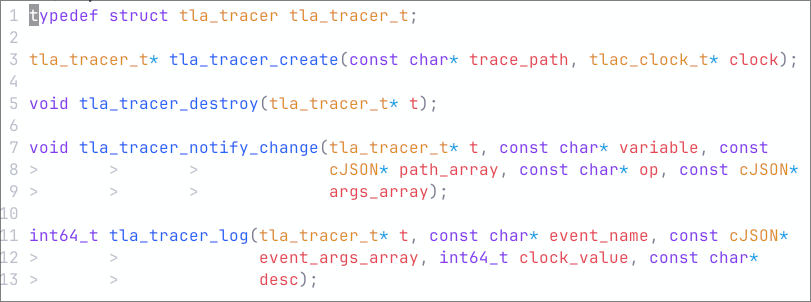
\includegraphics[scale=0.5]{inc/tlac-impl.png}
  \caption{Интерфейс библиотеки инструментирования реализации}
  \label{fig:tlac-impl}
\end{figure}

Для согласования порядка событий используется абстракция часов (см.
\texttt{tlac\_clock\_t} в функции \texttt{tla\_tracer\_create}). Часы могут
быть:
\begin{itemize}
    \item локальными (в памяти процесса),
    \item файловыми (для процессов на одном компьютере),
\end{itemize}

Все трассировщики синхронизируются через один и тот же механизм часов,
что обеспечивает монотонность временных меток как внутри одного процесса,
так и глобально между несколькими процессами. Возвращаемое функцией
\texttt{tla\_tracer\_log} значение --- это использованная временная метка.

Функция \texttt{tla\_tracer\_log} создаёт одну запись в файле трассы.
В запись включаются (см. рис~\ref{fig:json}):

\begin{itemize}
    \item временная метка (\texttt{"clock"});
    \item все изменения переменных, накопленные после предыдущего вызова
\texttt{log};
    \item имя события (\texttt{"event"});
    \item аргументы события (\texttt{"event\_args"}, например, ID узла).
\end{itemize}

После записи буфер изменений очищается. Таким образом, один вызов \texttt{log}
соответствует одному логическому шагу спецификации, объединяя несколько
изменений переменных в атомарную запись трассы.

В реализации допускается логирование только подмножества переменных
спецификации. В этом случае модельный проверяющий будет восстанавливать
отсутствующую информацию недетерминированным образом. Тем не менее, более
подробная трассировка (фиксация и переменных, и параметров действий)
существенно сокращает пространство поиска TLC и повышает достоверность
результатов валидации.

\begin{figure}
  \centering
  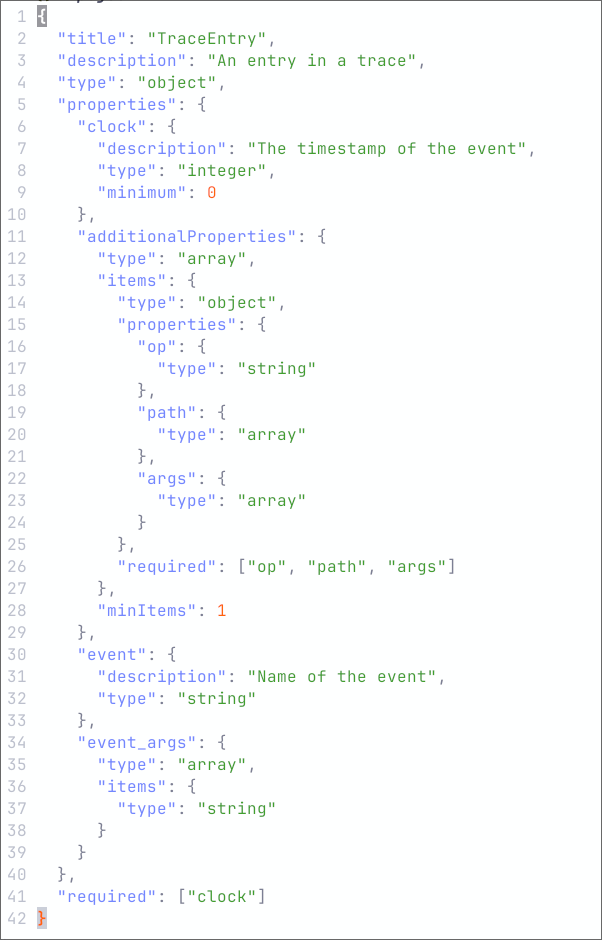
\includegraphics[scale=0.5]{inc/json.png}
  \caption{JSON структура записи трассы}
  \label{fig:json}
\end{figure}
